    \subsection{Recovery of the Schwarzschild Metric}
      \label{subsec:recovery-of-the-schwarzschild-metric}

      In the presence of a static and approximately spherically symmetric distribution
      of localized $\chi$ excitations, the collective slowdown of the relaxation flow
      admits a simple effective description.
      In the weak-coupling and quasi-static regime, the spatial variation of the
      relaxation rate can be summarized by a Poisson-like relation between the effective
      gravitational potential and the excitation density.

      When expressed in an effective geometric language, this structure is well
      described by a metric whose leading-order form coincides with the Schwarzschild
      solution of general relativity.
      In particular, the temporal and radial components of the effective metric encode
      the reduction of the local relaxation rate induced by the excitation, while the
      angular part reflects the isotropy of the configuration.

      Within this description, standard weak-field predictions of general relativity
      are recovered.
      These include gravitational redshift, light deflection, and time dilation effects
      consistent with solar-system observations.
      The gravitational constant $G$ appears as an emergent coupling parameter relating
      the density of localized excitations to the magnitude of the relaxation slowdown.

      \begin{figure}[htbp]
        \centering
        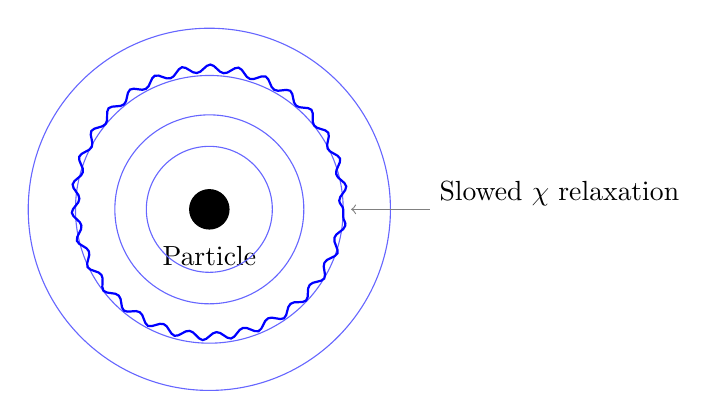
\begin{tikzpicture}[scale=1]

% Central mass
          \filldraw[black] (0,0) circle (0.25);
          \node[below] at (0,-0.35) {Particle};

% Phase lines
          \foreach \r in {0.8,1.2,1.7,2.3} {
            \draw[blue!60] (0,0) circle (\r);
          }

% Distortion
          \draw[blue, thick, decorate, decoration={snake, amplitude=0.5mm}]
          (0,0) circle (1.7);

% Arrows
          \draw[->, gray] (2.8,0) -- (1.8,0);
          \node[right] at (2.8,0.2) {Slowed $\chi$ relaxation};

        \end{tikzpicture}
        \caption
        {Emergence of gravity in Cosmochrony. Localized excitations of $\chi$ slow down the relaxation rate of the field
          ,inducing differential proper-time flow and an effective metric curvature analogous to gravitational time
        dilation.}
        \label{fig:chi_gravity}
      \end{figure}

      Importantly, the Schwarzschild metric is not postulated as a fundamental solution,
      nor is spacetime curvature treated as a primitive entity.
      Rather, the metric provides a compact and effective summary of how the collective
      dynamics of $\chi$ around a localized excitation constrains the relaxation flow.
      In this sense, Schwarzschild-like behavior emerges as a necessary phenomenological
      description in regimes where the relaxation field is close to local equilibrium.
